\tikzset{
    train/.style={
        text=black,
        draw,
        minimum height=1cm,
        minimum width=6cm,
        fill=RoyalBlue!30!white},
        % left color=royalblue!30!white, right color=orange!30!white,shading angle=90},
    val/.style={
        draw,
        text=black,
        minimum height=1cm,
        minimum width=2cm,
        fill=RoyalBlue!60!white},
        % left color=orange!60!white, right color=orange!60!white,shading angle=90},
    test/.style={
        draw,
        text=black,
        fill=RoyalBlue,
        minimum height=1cm,
        minimum width=2cm}}
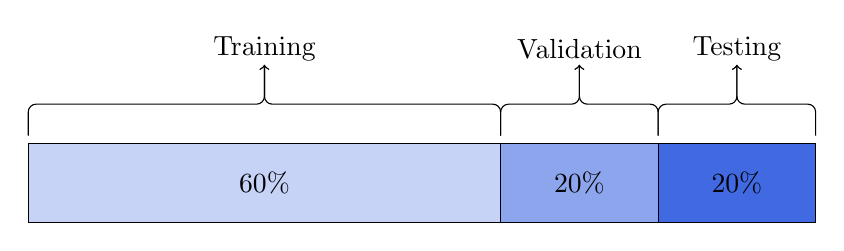
\begin{tikzpicture}[thin,black]
\path
(0,0)       node[train] (N) {60\%}
++(0:4)     node[val] (C) {20\%}
+(0:2)    node[test] (O) {20\%};
\draw[->,rounded corners=1mm] (-3.0,0.6) |- (0,1) -- ++(0,0.5);
\draw[->,rounded corners=1mm] (3.0,0.6) |- (0,1) -- ++(0,0.5);
\draw[->,rounded corners=1mm] (3.0,0.6) |- (4.0,1) -- ++(0,0.5);
\draw[->,rounded corners=1mm] (5.0,0.6) |- (4.0,1) -- ++(0,0.5);
\draw[->,rounded corners=1mm] (5,0.6) |- (6.0,1) -- ++(0,0.5);
\draw[->,rounded corners=1mm] (7,0.6) |- (6.0,1) -- ++(0,0.5);
\node at (0,1.7) {Training};
\node at (4.0,1.7) {Validation};
\node at (6.0,1.7) {Testing};
\end{tikzpicture} 